\section{Methodology}\label{sec:methodology}

This section formalizes the end-to-end research pipeline, from causal data preparation to environment transition mechanics and mask-aware value learning. To improve reproducibility, we provide explicit algorithmic specifications for (i) execution and portfolio updates, (ii) compositional reward assembly, and (iii) training-loop optimization; these correspond to Algorithms~\ref{alg:execution_portfolio_update}, \ref{alg:reward_computation}, and \ref{alg:mask_aware_training}, respectively.

\subsection{Design Principles and System Overview}
The methodology is organized around three design principles: \emph{economic fidelity}, \emph{temporal causality}, and \emph{auditability}. Economic fidelity is enforced through explicit transaction-cost and margin accounting; temporal causality is enforced through strict chronological processing and anti-lookahead execution timing; and auditability is enforced through deterministic component ordering, configuration snapshots, and structured logging artifacts. The resulting end-to-end pipeline (data ingestion $\rightarrow$ preprocessing $\rightarrow$ environment simulation $\rightarrow$ value-function learning $\rightarrow$ standardized evaluation export) is summarized in \Cref{fig:system_architecture}.

% Required in preamble:
%   \usepackage{tikz}
%   \usetikzlibrary{arrows.meta,positioning,fit,backgrounds,calc}
\usetikzlibrary{arrows.meta,positioning,fit,backgrounds,calc}

% ── Node & arrow style definitions ──────────────────────────────────────────
\tikzset{
  %-- module: processing / algorithmic component (blue)
  module/.style={
    draw=blue!55!black, line width=0.65pt,
    rounded corners=3pt,
    fill=blue!18,
    minimum height=9mm,
    text width=2.75cm,
    align=center,
    font=\footnotesize
  },
  %-- data: data store / artifact (green)
  data/.style={
    draw=green!55!black, line width=0.65pt,
    rounded corners=3pt,
    fill=green!18,
    minimum height=9mm,
    text width=2.75cm,
    align=center,
    font=\footnotesize
  },
  %-- subsystem: grouping box (dashed gray)
  subsystem/.style={
    draw=gray!55, line width=0.7pt,
    dashed,
    rounded corners=5pt,
    fill=gray!7,
    inner sep=14pt
  },
  %-- Arrow: data pipeline (solid green)
  dataarrow/.style={
    -{Latex[length=2.4mm,width=1.7mm]},
    line width=0.8pt,
    draw=green!55!black
  },
  %-- Arrow: agent <-> env interaction (solid blue)
  agentarrow/.style={
    -{Latex[length=2.4mm,width=1.7mm]},
    line width=0.8pt,
    draw=blue!60!black
  },
  %-- Arrow: logging / artifacts (dashed gray)
  logarrow/.style={
    -{Latex[length=2.4mm,width=1.7mm]},
    line width=0.7pt,
    dashed,
    draw=gray!55
  },
  %-- Arrow: general control / data flow (black)
  flowarrow/.style={
    -{Latex[length=2.4mm,width=1.7mm]},
    line width=0.8pt,
    draw=black!65
  }
}

% ── Figure ───────────────────────────────────────────────────────────────────
\begin{figure*}[!tbp]
\centering
% node distance = <vertical gap> and <horizontal gap>
% All gaps are measured between node borders (positioning library semantics).
\begin{tikzpicture}[node distance=9mm and 11mm]

% ─────────────────────────────────────────────────────────────────────────────
% ROW 1  ·  Experiment Configuration
% Two nodes, left-aligned with the data pipeline below.
% ─────────────────────────────────────────────────────────────────────────────
\node[data] (configs)
  {\textbf{configs/*}\\base, agents, features, exps};

\node[module, right=of configs] (runner)
  {\textbf{Experiment Runner}\\run\_experiment.py};

% ─────────────────────────────────────────────────────────────────────────────
% ROW 2  ·  Data Pipeline
% Four nodes spanning full width.  Col alignment is guaranteed because each
% node's text width is identical, so right=of advances by the same delta.
% ─────────────────────────────────────────────────────────────────────────────
\node[data,   below=20mm of configs] (raw)
  {\textbf{Raw Market Data}\\EURUSD, GBPUSD, USDJPY, AUDUSD};

\node[module, right=of raw] (prep)
  {\textbf{Loader \& Preprocess}\\clean, align, adjust};

\node[module, right=of prep] (feat)
  {\textbf{Feature Engineering}\\technical + microstructure};

\node[data,   right=of feat] (dataset)
  {\textbf{Dataset Builder}\\train\,,/\,test splits};

% ─────────────────────────────────────────────────────────────────────────────
% ROWS 3–4  ·  Training System (cols 1–2) + Evaluation (col 4)
% Anchoring env below raw AND backtest below dataset guarantees shared
% vertical levels for rows 3 and 4 on both sides of the diagram.
% ─────────────────────────────────────────────────────────────────────────────

%-- Training row 3
\node[module, below=20mm of raw] (env)
  {\textbf{Trading Env}\\execution + reward};

\node[module, right=of env] (agent)
  {\textbf{RL Agent}\\DQN\,/\,Double DQN};

%-- Evaluation row 3 (col 4, same vertical level as env/agent)
\node[module, below=20mm of dataset] (backtest)
  {\textbf{Backtest Engine}\\deterministic rollout};

%-- Training row 4
\node[module, below=9mm of env] (replay)
  {\textbf{Replay Buffer}\\experience memory};

\node[module, right=of replay] (trainer)
  {\textbf{Trainer}\\updates + target sync};

%-- Evaluation row 4 (col 4, same vertical level as replay/trainer)
\node[module, below=9mm of backtest] (metrics)
  {\textbf{Metrics}\\return, Sharpe, MDD};

% ─────────────────────────────────────────────────────────────────────────────
% ROW 5  ·  Logging & Artifacts
% ─────────────────────────────────────────────────────────────────────────────
\node[module, below=20mm of replay] (artifact)
  {\textbf{Artifact Manager}\\checkpoints, configs};

\node[module, right=of artifact] (logging)
  {\textbf{Logging}\\train/eval + TensorBoard};

\node[module, right=of logging] (repro)
  {\textbf{Reproducibility}\\seeding, diagnostics};

% ─────────────────────────────────────────────────────────────────────────────
% ARROWS
% ─────────────────────────────────────────────────────────────────────────────

%-- Experiment config / control flow ----------------------------------------
\draw[flowarrow] (configs) -- (runner);
% runner sits at col 2; prep also at col 2 → perfectly straight vertical
\draw[flowarrow] (runner.south) -- (prep.north);

%-- Data pipeline (solid green) ---------------------------------------------
\draw[dataarrow] (raw)  -- node[above,font=\footnotesize]{load}  (prep);
\draw[dataarrow] (prep) -- node[above,font=\footnotesize]{feats} (feat);
\draw[dataarrow] (feat) -- node[above,font=\footnotesize]{split} (dataset);

%-- Dataset → Evaluation: direct vertical (offset +1.5 mm to fork cleanly)
\draw[flowarrow] ([xshift=1.5mm]dataset.south)
  -- node[right,font=\footnotesize]{eval} ([xshift=1.5mm]backtest.north);

%-- Dataset → Training Env: western-margin bypass
%   Path: dataset.south  ─(down 5 mm into R2–R3 gap)─
%         ─(horizontal left to left-margin waypoint)─
%         ─(vertical down to env's y)─
%         ─(short horizontal right into env.west)
\coordinate (westEntry) at ($(env.west)+(-9mm,0)$);
\draw[flowarrow]
  ([xshift=-1.5mm]dataset.south)
  -- ++(0,-5mm)
  -| (westEntry)
  -- node[above,font=\footnotesize]{train} (env.west);

%-- Environment ↔ Agent: dual offset lanes (solid blue) --------------------
\draw[agentarrow]
  ([yshift= 2mm]env.east)
  -- node[above,font=\footnotesize,text=blue!65!black]{obs}
  ([yshift= 2mm]agent.west);

\draw[agentarrow]
  ([yshift=-2mm]agent.west)
  -- node[below,font=\footnotesize,text=blue!65!black]{action}
  ([yshift=-2mm]env.east);

%-- Training internals
\draw[flowarrow] (env.south)   -- (replay.north);
\draw[flowarrow] (replay.east) -- node[above,font=\footnotesize]{transitions} (trainer.west);
\draw[flowarrow] (agent.south) -- node[right,font=\footnotesize]{policy} (trainer.north);

%-- Evaluation chain
\draw[flowarrow] (backtest.south) -- node[right,font=\footnotesize]{stats} (metrics.north);

%-- Logging flows (dashed gray)
%   trainer → logging: offset +1.5 mm east, straight vertical
\draw[logarrow]
  ([xshift= 1.5mm]trainer.south)
  -- ++(0,-3mm)
  -| node[below right,font=\footnotesize]{log}
  (logging.north);

%   trainer → artifact: route through R4–R5 gap, then left to artifact
\draw[logarrow]
  ([xshift=-1.5mm]trainer.south)
  -- ++(0,-5mm)
  -| node[above,font=\footnotesize]{ckpt}
  (artifact.north);

%   metrics → logging: route through R4–R5 gap (staggered at −4.5 mm
%   to avoid the trainer→logging horizontal at −3 mm)
\draw[logarrow]
  (metrics.south)
  -- ++(0,-4.5mm)
  -| node[above,font=\footnotesize]{eval}
  (logging.east);

% ─────────────────────────────────────────────────────────────────────────────
% BACKGROUND SUBSYSTEM BOXES
% fit= auto-sizes each box; labels anchor inside the box border.
% ─────────────────────────────────────────────────────────────────────────────
\begin{scope}[on background layer]

  \node[subsystem,
    fit=(configs)(runner),
    label={[anchor=north west,font=\bfseries\footnotesize,text=black!70]
      north west:\strut 1.~Experiment Configuration}] {};

  \node[subsystem,
    fit=(raw)(prep)(feat)(dataset),
    label={[anchor=north west,font=\bfseries\footnotesize,text=black!70]
      north west:\strut 2.~Data Pipeline}] {};

  \node[subsystem,
    fit=(env)(agent)(replay)(trainer),
    label={[anchor=north west,font=\bfseries\footnotesize,text=black!70]
      north west:\strut 3.~Training System}] {};

  \node[subsystem,
    fit=(backtest)(metrics),
    label={[anchor=north west,font=\bfseries\footnotesize,text=black!70]
      north west:\strut 4.~Evaluation}] {};

  \node[subsystem,
    fit=(artifact)(logging)(repro),
    label={[anchor=north west,font=\bfseries\footnotesize,text=black!70]
      north west:\strut 5.~Logging \& Artifacts}] {};

\end{scope}

% ─────────────────────────────────────────────────────────────────────────────
% LEGEND
% Centered below Row 5, using the midpoint between leftmost and rightmost
% bottom nodes so the legend self-adjusts if nodes are added/removed.
% ─────────────────────────────────────────────────────────────────────────────
\node[
  draw=gray!50, rounded corners=3pt, fill=white,
  inner sep=7pt,
  font=\footnotesize,
  anchor=north,
] (legend) at ($(artifact.south)!0.5!(metrics.south)+(0,-24mm)$)
{%
  \renewcommand{\arraystretch}{1.18}%
  \begin{tabular}{@{}c@{\hspace{6pt}}l@{\hspace{14pt}}c@{\hspace{6pt}}l@{}}
    % ── Arrow types ──────────────────────────────────────────────────
    \begin{tikzpicture}[baseline=-0.5ex]
      \draw[dataarrow]  (0,0)--(10mm,0);
    \end{tikzpicture}
    & Data pipeline
    &
    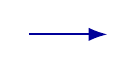
\begin{tikzpicture}[baseline=-0.5ex]
      \draw[agentarrow] (0,0)--(10mm,0);
    \end{tikzpicture}
    & Agent\,$\leftrightarrow$\,Env
    \\
    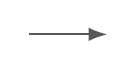
\begin{tikzpicture}[baseline=-0.5ex]
      \draw[flowarrow]  (0,0)--(10mm,0);
    \end{tikzpicture}
    & Control flow
    &
    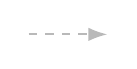
\begin{tikzpicture}[baseline=-0.5ex]
      \draw[logarrow]   (0,0)--(10mm,0);
    \end{tikzpicture}
    & Logging / artifact
    \\
    % ── Node types ───────────────────────────────────────────────────
    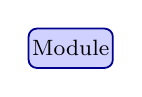
\begin{tikzpicture}[baseline=-0.5ex]
      \node[module, minimum height=5mm, text width=10mm,
          font=\footnotesize, inner sep=1pt]{Module};
    \end{tikzpicture}
    & Module (blue)
    &
    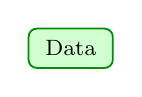
\begin{tikzpicture}[baseline=-0.5ex]
      \node[data, minimum height=5mm, text width=10mm,
          font=\footnotesize, inner sep=1pt]{Data};
    \end{tikzpicture}
    & Data node (green)
    \\
  \end{tabular}%
};

\end{tikzpicture}

\caption{System architecture of the RL trading framework, linking configuration, data processing, training, deterministic backtesting, and reproducibility logging in one end-to-end pipeline.}
\label{fig:system_architecture}

\end{figure*}

\subsection{Data Pipeline, Temporal Partitioning, and Leakage Control}
The dataset consists of hourly open-high-low-close-volume (OHLCV) bars for EURUSD, GBPUSD, USDJPY, and AUDUSD (summary in \Cref{tab:dataset}). Data are normalized to Coordinated Universal Time (UTC), validated for schema integrity, deduplicated using a last-occurrence retention policy, and processed with deterministic missing-value handling.


\paragraph{Chronological processing policy.}
To preserve temporal causality, all experiments process data in strict chronological order with no shuffling. All evaluation metrics are computed exclusively on training trajectories and logged artifacts. No held-out or test split is used at any stage. This ensures that all reported results reflect only the training distribution, with no claims regarding generalization or out-of-sample performance.

\paragraph{Train-only transformations and warm-up handling.}
Feature scaling parameters are estimated on the training data only and reused throughout. To initialize rolling indicators at the start of training, a warm-up lookback segment is prepended from the beginning of the training data, and warm-up rows are discarded from final training artifacts. No test or held-out data is used for any transformation or initialization.

\subsection{Feature Engineering and Observation Construction}
Features are organized into deterministic namespaces so that all runs share a stable, auditable column ordering:
\begin{itemize}[leftmargin=1.4em]
    \item \textbf{Technical indicators}: simple and exponential moving averages (SMA/EMA; 10, 20, 50), relative strength index (RSI; 14), moving average convergence divergence (MACD; 12, 26, 9), Bollinger components (20, $2\sigma$), one-bar log return, and rolling volatility.
	\item \textbf{Microstructure proxies}: spread proxy $(H-L)/C$, short-horizon price-change proxy, realized volatility proxy, and UTC session label.
\end{itemize}
The canonical ordering improves reproducibility and prevents accidental feature-index drift across experiment variants.

\paragraph{Windowing and input dimensions.}
Let $L$ denote the observation lookback window ($L=24$ in release runs), $d_{\mathrm{feat}}$ the number of engineered market features, $d_{\mathrm{port}}=10$ the portfolio-state dimension, and $n_a$ the active action count ($n_a \in \{3,10\}$). The flattened MLP input dimension is
\begin{equation}
d_{\mathrm{flat}} = L\,d_{\mathrm{feat}} + d_{\mathrm{port}} + n_a.
\label{eq:flat_input_dim}
\end{equation}
Equation~\ref{eq:flat_input_dim} is used consistently across training and evaluation to guarantee that architecture instantiation matches the declared observation schema.
The observation schema is summarized in \Cref{tab:obs_schema}.

\begin{table}[!tbp]
\centering
\caption{Observation schema and dimensions used by the Gymnasium environment.}
\label{tab:obs_schema}

\begin{adjustbox}{width=\linewidth}
\begin{tabularx}{\linewidth}{@{}l l X@{}}
\toprule
\textbf{Field} & \textbf{Shape} & \textbf{Role} \\
\midrule
\texttt{market} & $[L, d_{\mathrm{feat}}]$ & Rolling market-feature window ($L=24$) \\
\texttt{portfolio} & $[d_{\mathrm{port}}]$ & Normalized account state ($d_{\mathrm{port}}=10$) \\
\texttt{mask} & $[n_a]$ & Legal-action mask ($n_a\in\{3,10\}$) \\
\texttt{flat} & $[L d_{\mathrm{feat}} + d_{\mathrm{port}} + n_a]$ & Flattened vector for MLP agents \\
\bottomrule
\end{tabularx}
\end{adjustbox}
\end{table}



\subsection{Trading Environment}
The environment follows the Gymnasium application programming interface (API), consistent with the OpenAI Gym design lineage \citep{brockman2016openai}, and exposes dictionary observations together with deterministic transition diagnostics. This explicit state contract enables direct reproducibility checks across training and evaluation workflows.

\subsubsection{Action Space and Legal Masking}

The extended action interface contains 10 operations:
\begin{itemize}
    \item \texttt{HOLD}
    \item \texttt{OPEN\_LONG}, \texttt{OPEN\_SHORT}
    \item \texttt{PYRAMID\_LONG}, \texttt{PYRAMID\_SHORT}
    \item \texttt{MARTINGALE\_LONG}, \texttt{MARTINGALE\_SHORT}
    \item \texttt{REDUCE}
    \item \texttt{CLOSE}
    \item \texttt{REVERSE}
\end{itemize}

For controlled comparisons, a simplified 3-action adapter is used:
\begin{itemize}
    \item \texttt{HOLD}
    \item \texttt{TARGET\_LONG}
    \item \texttt{TARGET\_SHORT}
\end{itemize}
These are mapped to valid extended operations conditioned on the current position state.

Action legality is recomputed at every step using direction, margin availability, and scaling-depth constraints. The legal mask is stored with transitions in replay and reused for both exploratory sampling and masked argmax target computation. Although prior empirical evidence is reported primarily for policy-gradient settings \citep{huang2020closer}, the same legality principle is applied here to value-based updates. \Cref{tab:action_definitions} summarizes extended-action semantics.
\begin{table*}[!tbp]
\centering
\caption{Extended action semantics and legality conditions (executed at $open_{t+1}$).}
\label{tab:action_definitions}

\begin{tabularx}{\linewidth}{@{}r l >{\raggedright\arraybackslash}X >{\raggedright\arraybackslash}X@{}}
\toprule
\textbf{ID} & \textbf{Action} & \textbf{Primary legality precondition} & \textbf{Execution effect} \\
\midrule
0 & HOLD & Always legal & Maintain current position; no new order submitted \\
1 & OPEN\_LONG & Flat position and sufficient free margin & Open long exposure at base lot size \\
2 & OPEN\_SHORT & Flat position and sufficient free margin & Open short exposure at base lot size \\
3 & PYRAMID\_LONG & Existing long position, scaling depth below cap, margin available & Add to long position using configured pyramid increment \\
4 & PYRAMID\_SHORT & Existing short position, scaling depth below cap, margin available & Add to short position using configured pyramid increment \\
5 & MARTINGALE\_LONG & Existing long position, martingale depth below cap, margin available & Add long exposure after adverse movement using martingale scaling rule \\
6 & MARTINGALE\_SHORT & Existing short position, martingale depth below cap, margin available & Add short exposure after adverse movement using martingale scaling rule \\
7 & REDUCE & Non-flat position & Partially reduce current exposure (configured reduction fraction) \\
8 & CLOSE & Non-flat position & Fully close current position \\
9 & REVERSE & Non-flat position and sufficient margin for opposite side & Close current direction, then open opposite direction within one action \\
\bottomrule
\end{tabularx}
\end{table*}




\subsubsection{Execution Timing and Market Frictions}
To prevent lookahead leakage, step timing is fixed as:
\begin{equation}
\begin{aligned}
\mathrm{observe}\,\mathrm{close}_t \;\rightarrow\; \mathrm{decide}\,a_t \;\rightarrow\; \mathrm{fill}\,\mathrm{open}_{t+1} \\
\rightarrow\; \mathrm{mark}\,\mathrm{close}_{t+1}.
\end{aligned}
\label{eq:execution_timing_contract}
\end{equation}
The fill model applies spread, commission, and slippage in deterministic order; rollover financing is charged at 22:00~UTC with triple rollover on Wednesdays. Equation~\ref{eq:execution_timing_contract} is the causal timing contract summarized in \Cref{fig:timing_diagram}.

% ============================================================
%  fig03_timing_diagram.tex
%  Execution timing diagram for one RL trading environment step.
%  Causality-correct sequence diagram with explicit time axis.
%  Requires: tikz with libraries arrows.meta, positioning,
%            fit, backgrounds, calc
% ============================================================
\usetikzlibrary{arrows.meta,positioning,fit,backgrounds,calc}

% ------------------------------------------------------------------
%  Style definitions
% ------------------------------------------------------------------
\tikzset{
    actor/.style={
        draw=blue!55!black,
        fill=blue!12,
        rounded corners=3pt,
        minimum width=2.15cm,
        minimum height=9mm,
        align=center,
        font=\footnotesize\bfseries
    },
    lifeline/.style={
        dashed,
        draw=black!40,
        line width=0.5pt
    },
    event/.style={
        draw=green!50!black,
        fill=green!10,
        rounded corners=3pt,
        minimum width=2.10cm,
        minimum height=8mm,
        align=center,
        font=\footnotesize
    },
    arr/.style={
        -{Latex[length=2.2mm,width=1.6mm]},
        line width=0.85pt,
        draw=black!75
    },
    boundary/.style={
        draw=orange!75!black,
        dotted,
        line width=0.9pt
    },
    timeline/.style={
        -{Latex[length=2.4mm,width=1.7mm]},
        draw=black!70,
        line width=0.75pt
    },
    timetick/.style={
        draw=black!65,
        line width=0.55pt
    },
    msglabel/.style={
        font=\scriptsize,
        inner sep=1.2pt,
        fill=white,
        align=center
    },
    delaylabel/.style={
        font=\scriptsize\itshape,
        text=purple!65!black,
        fill=white,
        inner sep=1pt
    }
}

% ------------------------------------------------------------------
%  Diagram geometry
% ------------------------------------------------------------------
\newcommand{\COLSEP}{2.20cm}  % centre-to-centre actor spacing

\def\Yone{1.15}
\def\Ytwo{2.25}
\def\Ythree{3.35}
\def\Yfour{4.45}
\def\Yfive{5.55}
\def\Ysix{6.65}
\def\Yseven{7.75}
\def\Yeight{8.85}
\def\Ynine{9.95}
\def\Yten{11.05}
\def\YBOUND{5.00}
\def\LIFEBOT{11.85}

\begin{figure*}[!tbp]
\centering
\begin{tikzpicture}[
    x=1cm,
    y=-1cm,
    node distance=0pt
]

% ==================================================================
% ACTOR HEADER ROW
% ==================================================================
\node[actor] (A_market)    at (0*\COLSEP,0) {Market\\Simulator};
\node[actor] (A_env)       at (1*\COLSEP,0) {TradingEnv};
\node[actor] (A_agent)     at (2*\COLSEP,0) {RL Agent};
\node[actor] (A_exec)      at (3*\COLSEP,0) {Execution\\Model};
\node[actor] (A_portfolio) at (4*\COLSEP,0) {Portfolio\\System};
\node[actor] (A_reward)    at (5*\COLSEP,0) {Reward\\Engine};

% ==================================================================
% LIFELINES
% ==================================================================
\foreach \actor in {A_market,A_env,A_agent,A_exec,A_portfolio,A_reward}{
    \draw[lifeline] (\actor.south) -- ($(\actor.south)+(0,\LIFEBOT)$);
}

% Coordinates on lifelines (structural timing grid)
\foreach \r/\y in {
    r1/\Yone,
    r2/\Ytwo,
    r3/\Ythree,
    r4/\Yfour,
    r5/\Yfive,
    r6/\Ysix,
    r7/\Yseven,
    r8/\Yeight,
    r9/\Ynine,
    r10/\Yten
}{
    \coordinate (mkt-\r) at ($(A_market.south)+(0,\y)$);
    \coordinate (env-\r) at ($(A_env.south)+(0,\y)$);
    \coordinate (agt-\r) at ($(A_agent.south)+(0,\y)$);
    \coordinate (exe-\r) at ($(A_exec.south)+(0,\y)$);
    \coordinate (pf-\r)  at ($(A_portfolio.south)+(0,\y)$);
    \coordinate (rew-\r) at ($(A_reward.south)+(0,\y)$);
}

% ==================================================================
% TIME AXIS + TICKS (explicit temporal reference)
% ==================================================================
\coordinate (TimeTop) at ($(A_market.west)+(-1.25cm,0.35)$);
\draw[timeline] (TimeTop) -- ($(TimeTop)+(0,\LIFEBOT+0.25)$)
    node[below,font=\footnotesize] {time $\tau$};

\coordinate (T1) at (TimeTop |- mkt-r1);
\coordinate (T2) at (TimeTop |- agt-r3);
\coordinate (T3) at (TimeTop |- mkt-r5);
\coordinate (T4) at (TimeTop |- mkt-r8);
\coordinate (T5) at (TimeTop |- env-r10);

\draw[timetick] ($(T1)+(-0.09,0)$) -- ($(T1)+(0.09,0)$);
\draw[timetick] ($(T2)+(-0.09,0)$) -- ($(T2)+(0.09,0)$);
\draw[timetick] ($(T3)+(-0.09,0)$) -- ($(T3)+(0.09,0)$);
\draw[timetick] ($(T4)+(-0.09,0)$) -- ($(T4)+(0.09,0)$);
\draw[timetick] ($(T5)+(-0.09,0)$) -- ($(T5)+(0.09,0)$);

\node[anchor=west,font=\scriptsize] at ($(T1)+(0.13,0)$) {$\tau_0$};
\node[anchor=west,font=\scriptsize] at ($(T2)+(0.13,0)$) {$\tau_2$};
\node[anchor=west,font=\scriptsize] at ($(T3)+(0.13,0)$) {$\tau_4$};
\node[anchor=west,font=\scriptsize] at ($(T4)+(0.13,0)$) {$\tau_6$};
\node[anchor=west,font=\scriptsize] at ($(T5)+(0.13,0)$) {$\tau_8$};

% ==================================================================
% CAUSAL BOUNDARY (horizontal: separates t from t+1 market info)
% ==================================================================
\draw[boundary]
    ($(A_market.west)+(-0.55cm,\YBOUND)$) -- ($(A_reward.east)+(0.55cm,\YBOUND)$)
    node[pos=1,above,anchor=east,font=\footnotesize,text=orange!80!black,fill=white,inner sep=1.3pt]
    {causal boundary $t\mid t{+}1$ (anti-lookahead)};

% ==================================================================
% EVENT FLOW (causality-correct MDP transition)
% ==================================================================
\node[event] (E_close_t) at (mkt-r1)
    {publish\\$\mathrm{close}_t$};
\draw[arr] (E_close_t.east) -- node[msglabel,above] {$\mathrm{close}_t$} (env-r1);

\node[event] (E_state_t) at (env-r2)
    {build state\\$\mathbf{s}_t$};
\draw[arr] (E_state_t.east) -- node[msglabel,above] {$\mathbf{s}_t$} (agt-r2);

\node[event] (E_action) at (agt-r3)
    {policy step\\$a_t\in\{-1,0,+1\}$};
\draw[arr] (E_action.west) -- node[msglabel,above] {$a_t$} (env-r3);

\node[event] (E_order) at (env-r4)
    {validate + queue\\order$_t$};
\draw[arr] (E_order.east) -- node[msglabel,above] {order$_t$} (exe-r4);

\node[delaylabel] at ($(exe-r4)!0.5!(exe-r5)+(0.62,0)$) {$\Delta\tau_{\text{route}}$};

\node[event] (E_open_tp1) at (mkt-r5)
    {publish\\$\mathrm{open}_{t+1}$};
\draw[arr] (E_open_tp1.east) -- node[msglabel,above] {$\mathrm{open}_{t+1}$ feed} (exe-r5);

\node[event] (E_fill) at (exe-r6)
    {match + slippage\\execution fill};
\draw[arr] (E_fill.east) -- node[msglabel,above] {fill report} (pf-r7);

\node[event] (E_portfolio) at (pf-r7)
    {apply fees\\update position};

\node[event] (E_close_tp1) at (mkt-r8)
    {publish\\$\mathrm{close}_{t+1}$};
\draw[arr] (E_close_tp1.east) -- node[msglabel,above] {$\mathrm{close}_{t+1}$} (pf-r8);
\draw[arr] (E_close_tp1.east) -- node[msglabel,below] {market obs$_{t+1}$} (env-r8);

\node[event] (E_mark) at (pf-r8)
    {mark-to-market\\$\Delta\mathrm{PnL}_{t+1}$};
\draw[arr] (E_mark.east) -- node[msglabel,above] {$\Delta\mathrm{PnL}$, costs} (rew-r9);

\node[event] (E_reward) at (rew-r9)
    {compute reward\\$r_t$};
\draw[arr] (E_reward.west) -- node[msglabel,above] {$r_t$} (env-r9);

\node[delaylabel] at ($(env-r9)!0.5!(env-r10)+(-0.60,0)$) {$\Delta\tau_{\text{env}}$};

\node[event] (E_transition) at (env-r10)
    {build $\mathbf{s}_{t+1}$\\emit transition};
\draw[arr] (E_transition.east)
    -- node[msglabel,above] {$(\mathbf{s}_t,a_t,r_t,\mathbf{s}_{t+1})$}
    (agt-r10);

% ==================================================================
% BACKGROUND PHASE SHADING
% ==================================================================
\begin{scope}[on background layer]
    \fill[blue!4,rounded corners=4pt]
        ($(A_market.west)+(-0.55cm,0.55)$)
        rectangle
        ($(A_exec.east)+(0.55cm,4.92)$);

    \fill[green!4,rounded corners=4pt]
        ($(A_market.west)+(-0.55cm,5.08)$)
        rectangle
        ($(A_reward.east)+(0.55cm,\LIFEBOT)$);
\end{scope}

\node[
    font=\footnotesize\itshape,
    text=blue!60!black,
    align=left,
    anchor=west
] at ($(TimeTop)+(0.22,2.55)$) {Bar $t$\\(observe + decide)};

\node[
    font=\footnotesize\itshape,
    text=green!55!black,
    align=left,
    anchor=west
] at ($(TimeTop)+(0.22,7.95)$) {Bar $t{+}1$\\(execute + settle)};

\end{tikzpicture}

\caption{Causality-correct environment step timing: the environment emits $\mathbf{s}_t$, receives $a_t$, execution is driven by market $\mathrm{open}_{t+1}$, portfolio state is marked at $\mathrm{close}_{t+1}$, reward engine returns only $r_t$ to the environment, and the environment emits the full transition $(\mathbf{s}_t,a_t,r_t,\mathbf{s}_{t+1})$ without any Reward$\rightarrow$Agent bypass.}
\label{fig:timing_diagram}
\end{figure*}

\subsubsection{Portfolio and Risk Accounting}
The account model tracks cash, equity, realized and unrealized PnL, used/free margin, directional exposure, scaling depth, and drawdown. Core constraints include maximum leverage ($30\times$), maintenance margin ($50\%$ of initial margin requirement), bounded scaling depth, and forced liquidation at a fixed equity threshold. These controls are necessary to prevent value-function optimization from exploiting infeasible leverage trajectories.

Algorithm~\ref{alg:execution_portfolio_update} formalizes the exact execution and accounting order, including legality checks, friction application, rollover timing, margin updates, and forced liquidation handling.

\begin{algorithm}[!tbp]
\caption{Execution and portfolio update with frictions.}
\label{alg:execution_portfolio_update}
\begin{algorithmic}[1]
\STATE \textbf{Input:} portfolio state $P_t$, action proposal $a_t$, bars
\STATE \hspace*{1em} $(\mathrm{close}_t,\mathrm{open}_{t+1},\mathrm{close}_{t+1})$, configuration $\Omega$, legal mask $m_t$
\STATE \textbf{Output:} next portfolio state $P_{t+1}$, realized/unrealized PnL,
\STATE \hspace*{1em} cost trace, violation flag, and liquidation flag
\STATE Recompute $m_t$ from current direction, free margin, and scaling-depth limits
\IF{$m_t[a_t]=0$}
    \STATE Set executed action $\tilde{a}_t \leftarrow \texttt{HOLD}$ and raise constraint-violation flag
\ELSE
    \STATE Set $\tilde{a}_t \leftarrow a_t$
\ENDIF
\STATE Perform pre-trade feasibility checks for $\tilde{a}_t$ (margin and leverage)
\IF{pre-trade feasibility fails}
    \STATE Set $\tilde{a}_t \leftarrow \texttt{HOLD}$ and raise constraint-violation flag
\ENDIF
\STATE Set base execution anchor $p_{\mathrm{base}} \leftarrow \mathrm{open}_{t+1}$
\STATE Apply spread adjustment to obtain side-aware quoted price
\STATE Apply deterministic slippage to obtain final fill price $p_{\mathrm{fill}}$
\STATE Execute action semantics for $\tilde{a}_t$ (open, scale, reduce, close, reverse, or hold)
\STATE Deduct commissions from cash according to traded volume
\IF{timestamp equals rollover time (22:00 UTC)}
    \STATE Apply rollover financing (triple rollover on Wednesday)
\ENDIF
\STATE Mark open positions to $\mathrm{close}_{t+1}$ and update unrealized and realized PnL
\STATE Update cash, equity, used/free margin, utilization ratio, and drawdown statistics
\IF{equity below liquidation threshold \textbf{or} maintenance-margin rule violated}
    \STATE Force-liquidate all open positions using configured liquidation convention
    \STATE Set liquidation event flag and apply liquidation accounting effects
\ENDIF
\STATE Construct and return $P_{t+1}$ with per-step diagnostic traces
\end{algorithmic}
\end{algorithm}


\subsection{Compositional Reward Modeling}

We model the reward as a weighted composition of components. Let $c_i(s_t, a_t, s_{t+1})$ denote component $i$ with weight $w_i$. The pre-normalized reward is:
\begin{equation}
R_t^{\text{raw}} = \sum_{i=1}^{11} w_i\, c_i(s_t, a_t, s_{t+1}).
\label{eq:raw_reward_sum}
\end{equation}
The final reward applies clipping:
\begin{equation}
R_t = \mathrm{clip}(R_t^{\text{raw}}, -1, 1).
\label{eq:reward_clip}
\end{equation}
Equation~\ref{eq:raw_reward_sum} defines deterministic component aggregation, and Equation~\ref{eq:reward_clip} bounds temporal-difference target magnitude.

\paragraph{Clipping vs. running normalization.}
Clipping bounds temporal-difference targets and stabilizes early training by limiting extreme updates. It preserves sign information and relative ordering within the unclipped region, but compresses large-magnitude rewards. In contrast, running normalization mitigates scale drift but introduces non-stationarity into the learning objective. We therefore adopt clipping as the default and use adaptive normalization only in sensitivity analyses.

\paragraph{Component structure and weighting.}
The 11 components span four functional groups: 
(i) return (post-cost profit), 
(ii) risk control (volatility and drawdown), 
(iii) trading frictions (transaction cost and overtrading), and 
(iv) constraints (margin usage, liquidation, and rule violations), 
with asymmetric penalties for scaling behaviors (martingale penalized more strongly than pyramiding). 
Baseline weights and definitions are provided in \Cref{tab:reward_components}.

\begin{table*}[!tbp]
\centering
\caption{Reward component definitions, baseline weights, and intended behavioral effect.}
\label{tab:reward_components}

\begin{adjustbox}{width=\linewidth}
\begin{tabular}{l r p{4.2cm} p{6.2cm}}
\toprule
\textbf{Component} & \textbf{Weight} & \textbf{Primary purpose} & \textbf{Typical trigger / penalty form} \\
\midrule
Profit (post-cost) & 1.00 & Core economic learning signal & Step-wise post-cost equity return \\
Holding incentive & 0.03 & Encourage controlled profitable holding & Small bonus when position remains profitable under low drawdown \\
Volatility penalty & 0.01 & Discourage unstable equity trajectories & Negative term proportional to short-horizon equity-return volatility \\
Drawdown penalty & 0.05 & Penalize increasing downside risk & Incremental drawdown penalty with stronger regime beyond severe drawdown threshold \\
Transaction burden & 0.10 & Reduce excessive cost-churning behavior & Cost-normalized penalty for spread, slippage, commission, and rollover \\
Overtrading penalty & 0.02 & Suppress unnecessary action frequency & Bounded penalty tied to elevated local trade frequency \\
Pyramiding penalty & 0.05 & Constrain winner-adding aggressiveness & Depth-aware penalty for additional pyramid levels \\
Martingale penalty & 0.12 & Strongly discourage loss-amplifying averaging down & Depth-aware penalty with larger coefficient than pyramiding \\
Margin-utilization penalty & 0.05 & Avoid extreme leverage usage before liquidation & Nonlinear penalty when utilization exceeds conservative threshold \\
Liquidation penalty & 2.00 & Impose catastrophic-event aversion & Large penalty on forced liquidation event \\
Constraint-violation penalty & 0.10 & Deter illegal action proposals & Penalty when policy attempts an invalid action \\
\bottomrule
\end{tabular}
\end{adjustbox}
\end{table*}




Algorithm~\ref{alg:reward_computation} specifies the deterministic per-step reward assembly pipeline, including component enable switches for ablations, weighting, clipping, and structured logging.

\begin{algorithm}[!tbp]
\caption{Per-step compositional reward computation.}
\label{alg:reward_computation}
\begin{algorithmic}[1]
\STATE \textbf{Input:} transition trace $\tau_t$, component enable switches $g_i \in \{0,1\}$,
\STATE \hspace*{1em} weights $w_i$, clipping bounds $[r_{\min},r_{\max}]$
\STATE \textbf{Output:} clipped reward $r_t$ and component log dictionary $\mathcal{L}_t$
\STATE Define fixed component order:
\STATE \hspace{1em}profit, holding, volatility, drawdown, transaction, overtrading,
\STATE \hspace{1em}pyramiding, martingale, margin-utilization, liquidation, constraint-violation
\FOR{each component $i$ in the fixed order}
    \IF{$g_i=1$}
        \STATE Compute component value $c_i(\tau_t)$
    \ELSE
        \STATE Set $c_i(\tau_t) \leftarrow 0$
    \ENDIF
    \STATE Compute weighted term $u_i \leftarrow w_i\,c_i(\tau_t)$
    \STATE Append $(c_i,w_i,u_i,g_i)$ to $\mathcal{L}_t$
\ENDFOR
\STATE Compute raw reward $r_t^{\mathrm{raw}} \leftarrow \sum_i u_i$
\STATE Compute clipped reward $r_t \leftarrow \mathrm{clip}(r_t^{\mathrm{raw}}, r_{\min}, r_{\max})$
\STATE Append $(r_t^{\mathrm{raw}}, r_t, \mathbb{1}[r_t^{\mathrm{raw}} \neq r_t])$ to $\mathcal{L}_t$
\STATE Return $(r_t,\mathcal{L}_t)$
\end{algorithmic}
\end{algorithm}


\paragraph{Logging and ablation protocol.}
Component evaluation follows a fixed order, and each term is logged per step via the environment \texttt{info} dictionary and persisted reward traces. This enables direct attribution in ablation experiments (\variant{r1}--\variant{r7}), where individual components or weights are selectively modified. Because non-potential reward shaping can alter optimal policies \citep{ng1999policy}, profit remains the primary signal, with auxiliary penalties introduced incrementally.

\usetikzlibrary{arrows.meta,positioning,matrix}

\newcommand{\nodepair}[2]{\textbf{#1}\\\footnotesize #2}

\tikzset{
base node/.style={
draw=black!68,
thick,
rounded corners=2.5pt,
align=center,
font=\footnotesize,
inner sep=3pt,
minimum height=8.5mm,
text width=2.15cm
},
module/.style={base node, fill=blue!12},
data/.style={base node, fill=green!12, text width=2.05cm},
component/.style={base node, fill=yellow!18, text width=2.25cm},
flowarrow/.style={-{Latex[length=2.1mm,width=1.7mm]}, semithick, draw=black!72},
rewardarrow/.style={-{Latex[length=2.5mm,width=2.0mm]}, very thick, draw=black!90},
controlarrow/.style={-{Latex[length=2.0mm,width=1.6mm]}, thin, draw=blue!60!black!75},
edgelabel/.style={font=\footnotesize, fill=white, inner sep=1pt, rounded corners=1pt}
}

\begin{figure*}[!tbp]
\centering
\begin{tikzpicture}[node distance=11mm and 14mm]

% ========== ROW 1: AGENT INTERACTION ==========
\node[module] (agent) {\nodepair{Agent / Policy}{action selection}};
\node[module, right=of agent] (envstep) {\nodepair{Env.step}{transition + reward}};

% ========== ROW 2: EXECUTION & PORTFOLIO ==========
\node[module, below=of envstep] (exec) {\nodepair{Execution Model}{fills, slippage, fees}};
\node[module, right=of exec] (pos) {\nodepair{Position Manager}{entry / exit / pyramid}};
\node[module, right=of pos] (portfolio) {\nodepair{Portfolio Manager}{cash, pnl, margin}};

\matrix (sharedinputs) [matrix of nodes,
nodes={data},
column sep=16mm,
below=of portfolio,
anchor=north] {
|[alias=state]|{\nodepair{State}{PortfolioState $s_t, s_{t-1}$}} &
|[alias=cost]|{\nodepair{Cost Terms}{fees, slippage, impact}} \\
};

% ========== ROW 3: REWARD COMPONENTS GRID (CENTRAL FOCAL BLOCK) ==========
\matrix (rewardgrid) [matrix of nodes,
nodes={component},
column sep=5mm,
row sep=3.5mm,
below=of sharedinputs,
anchor=north] {
|[alias=pnl]|         {\nodepair{Profit}{PnL reward}} &
|[alias=transaction]| {\nodepair{Transaction}{turnover penalty}} \\
|[alias=vol]|         {\nodepair{Volatility}{risk penalty}} &
|[alias=drawdown]|    {\nodepair{Drawdown}{peak-to-trough penalty}} \\
|[alias=holding]|     {\nodepair{Holding}{stability incentive}} &
|[alias=overtrade]|   {\nodepair{Overtrading}{churn penalty}} \\
|[alias=scaling]|     {\nodepair{Scaling}{position-size penalty}} &
|[alias=margin]|      {\nodepair{Margin}{utilization penalty}} \\
|[alias=liq]|         {\nodepair{Liquidation}{hard-risk penalty}} &
|[alias=constraint]|  {\nodepair{Constraint}{violation penalty}} \\
};

% ========== ROW 4: REWARD AGGREGATION ==========
\node[module, below=of rewardgrid] (sum) {\nodepair{Weighted Sum}{component-weighted combination}};
\node[module, below=of sum] (norm) {\nodepair{Reward Normalizer}{clip / tanh / scale}};
\node[module, below=of norm] (final) {\nodepair{final\_reward}{scalar reward $r_t$}};

% ========== PRIMARY TOP-TO-BOTTOM FLOW ==========
\draw[controlarrow] (agent) -- node[edgelabel, above] {$a_t$} (envstep);
\draw[flowarrow] (envstep) -- (exec);
\draw[flowarrow] (exec) -- (pos);
\draw[flowarrow] (pos) -- (portfolio);
\draw[flowarrow] (portfolio.south) |- (state.north);
\draw[flowarrow] (portfolio.south) |- (cost.north);

\draw[flowarrow] (state.south) -- (rewardgrid.north west);
\draw[flowarrow] (cost.south) -- (rewardgrid.north east);
\node[edgelabel, above=1.5mm of sharedinputs.north] {shared inputs};

% Dominant reward computation path
\draw[rewardarrow] (rewardgrid.south) -- node[edgelabel, right] {10 components} (sum.north);
\draw[rewardarrow] (sum) -- node[edgelabel, right] {$\sum_i w_i r_i$} (norm);
\draw[rewardarrow] (norm) -- node[edgelabel, right] {$r_t$} (final);

% Secondary feedback (de-emphasized)
\draw[controlarrow] (final.west) to[out=165,in=-70] node[edgelabel, left] {$r_t$} (agent.south);

\end{tikzpicture}

\caption{Reward taxonomy and computation flow for the RL trading environment, from agent--environment interaction through component aggregation and normalization to the final scalar reward.}\label{fig:reward_taxonomy}
\end{figure*}
% Ensure floats from this section are placed here (prevent deferral into appendix)
\subsection{Agent Architectures}
Both agents are value-based and share the same backbone: a feed-forward multilayer perceptron (MLP) with hidden dimensions $[512,512,256]$, ReLU activations, and a linear Q-value output head. Output dimensionality equals the active action-space size ($3$ in simplified mode, $10$ in extended mode). The agents are Deep Q-Network (DQN) and Double Deep Q-Network (DDQN) variants, selected because they support explicit legality masking in discrete control.

\subsubsection{DQN}
DQN uses temporal-difference targets with periodic hard target-network synchronization \citep{mnih2015humanlevel}:
\begin{equation}
y_t^{\text{DQN}} = r_t + \gamma (1-d_t)\max_{a' \in \mathcal{A}_{\text{legal}}(s_{t+1})} Q_{\theta^-}(s_{t+1}, a').
\label{eq:dqn_target}
\end{equation}
Equation~\ref{eq:dqn_target} masks invalid actions directly in target construction.

\subsubsection{Double DQN}
Double DQN decouples action selection and evaluation:
\begin{equation}
a^* = \arg\max_{a' \in \mathcal{A}_{\text{legal}}(s_{t+1})} Q_{\theta}(s_{t+1}, a').
\label{eq:ddqn_action_select}
\end{equation}
\begin{equation}
y_t^{\text{DDQN}} = r_t + \gamma (1-d_t) Q_{\theta^-}(s_{t+1}, a^*).
\label{eq:ddqn_target}
\end{equation}
Equations~\ref{eq:ddqn_action_select} and \ref{eq:ddqn_target} separate online action selection from target-network evaluation, reducing value overestimation in volatile training regimes \citep{hasselt2016deep}.

\paragraph{Mask-aware exploration policy.}
Exploration follows an $\epsilon$-greedy policy defined on legal actions only: with probability $\epsilon$, the agent samples uniformly from legal actions; otherwise, it selects the legal argmax action. The same legality constraints are applied during replay-based target computation, ensuring consistency between data collection and value updates.

\paragraph{Algorithmic variants outside release scope.}
The architecture is compatible with dueling heads and distributional value estimation, which are relevant in heavy-tailed return settings \citep{wang2016dueling,bellemare2017distributional}. These variants are intentionally excluded from the main release protocol to isolate the effect of environment and reward design under DQN-family baselines.

\subsection{Training Protocol}
Core settings are fixed across experiment families unless explicitly overridden. For global reproducibility and side-by-side comparability, the exact training and environment values are consolidated in \Cref{tab:hyperparams} within \Cref{sec:experiments}.

Algorithm~\ref{alg:mask_aware_training} summarizes the full mask-aware DQN/DDQN training loop, including replay storage of legality masks, learn/start frequency gates, target-network synchronization, and periodic evaluation cadence.

\begin{algorithm}[!tbp]
\caption{Mask-aware DQN/DDQN training with legal-action masking.}
\label{alg:mask_aware_training}
\begin{algorithmic}[1]
\STATE \textbf{Input:}
\STATE \hspace*{1em} \textbf{Environment \,\& state:} environment $\mathcal{E}$; state $s_t$; legal-action mask $m_t \in \{0,1\}^{|\mathcal{A}|}$, where $m_t[a]=1$ iff $a$ is legal in $s_t$
\STATE \hspace*{1em} \textbf{Networks:} online network $Q_{\theta}$; target network $Q_{\theta^-}$
\STATE \hspace*{1em} \textbf{Replay buffer:} $\mathcal{D}$ with capacity $N$
\STATE \hspace*{1em} \textbf{Training hyperparameters:} batch size $B$; discount $\gamma$
\STATE \hspace*{1em} \textbf{Scheduling:} learn-start $t_{\mathrm{start}}$; learn frequency $f_{\mathrm{learn}}$; target-sync interval $f_{\mathrm{target}}$; evaluation interval $f_{\mathrm{eval}}$; total steps $T$; evaluation budget $K_{\mathrm{eval}}$
\STATE \hspace*{1em} \textbf{Algorithm type:} $\texttt{DQN}$ or $\texttt{DDQN}$
\STATE Initialize $\theta$ randomly; set $\theta^- \leftarrow \theta$; initialize the $\epsilon$ schedule
\STATE Reset $\mathcal{E}$ and observe $(s_0,m_0)$
\FOR{$t=0$ to $T-1$}
    \STATE Select $a_t$ by mask-aware $\epsilon$-greedy on $m_t$: with probability $\epsilon$, sample $a_t \sim \mathrm{Unif}(\{a:m_t[a]=1\})$; otherwise $a_t \leftarrow \arg\max_{a:\,m_t[a]=1} Q_{\theta}(s_t,a)$
    \STATE Execute $a_t$ in $\mathcal{E}$ and observe $(s'_{t},r_t,d_t,\mathrm{info}_t,m'_{t})$
    \STATE Store $(s_t,a_t,r_t,s'_{t},d_t,m_t,m'_{t})$ in $\mathcal{D}$
    \STATE Update $(s_t,m_t) \leftarrow (s'_{t},m'_{t})$
    \IF{$t \ge t_{\mathrm{start}}$ \textbf{and} $t \bmod f_{\mathrm{learn}}=0$ \textbf{and} $|\mathcal{D}| \ge B$}
        \STATE Sample minibatch $\{(s_i,a_i,r_i,s'_i,d_i,m_i,m'_i)\}_{i=1}^{B}$ from $\mathcal{D}$
        \IF{algorithm type is \texttt{DDQN}}
            \STATE $a_i^{\star} \leftarrow \arg\max_{a:\,m'_i[a]=1} Q_{\theta}(s'_i,a),\ \forall i$
            \STATE $y_i \leftarrow r_i + \gamma(1-d_i)Q_{\theta^-}(s'_i,a_i^{\star}),\ \forall i$
        \ELSE
            \STATE $y_i \leftarrow r_i + \gamma(1-d_i)\max_{a:\,m'_i[a]=1} Q_{\theta^-}(s'_i,a),\ \forall i$
        \ENDIF
        \STATE $\mathcal{L} \leftarrow \frac{1}{B}\sum_{i=1}^{B}\mathrm{Huber}\big(Q_{\theta}(s_i,a_i)-y_i\big)$
        \STATE Update $\theta$ by gradient descent with gradient clipping
    \ENDIF
    \IF{$t \bmod f_{\mathrm{target}}=0$}
        \STATE Hard-sync target network: $\theta^- \leftarrow \theta$
    \ENDIF
    \IF{$t \bmod f_{\mathrm{eval}}=0$}
        \STATE Evaluate the deterministic policy ($\epsilon=0$) for $K_{\mathrm{eval}}$ episodes and log all outputs
    \ENDIF
    \STATE Update $\epsilon$
\ENDFOR
\STATE \textbf{Output:} trained parameters $\theta$, replay buffer state, and diagnostic artifacts
\end{algorithmic}
\end{algorithm}

\usetikzlibrary{arrows.meta,positioning}

\tikzset{
loopnode/.style={
  draw=black!75,
  thick,
  rounded corners=2pt,
  fill=blue!6,
  align=center,
  font=\footnotesize,
  minimum width=2.85cm,
  minimum height=8mm
},
looparrow/.style={
  -{Latex[length=2.5mm,width=2mm]},
  thick,
  draw=black!75
}
}

\begin{figure}[!tbp]
\centering
\begin{tikzpicture}[node distance=8mm and 5mm]

\node[loopnode] (obs) {Build $s_t$, mask $m_t$};
\node[loopnode, below=of obs] (act) {Mask-aware $\epsilon$-greedy action};
\node[loopnode, below=of act] (step) {Env step ($t \to t+1$)};
\node[loopnode, below=of step] (next) {Compute $r_t$, $s_{t+1}$,\\mask $m_{t+1}$};
\node[loopnode, below=of next] (store) {Store transition};
\node[loopnode, below=of store] (learn) {Sample replay +\\masked Q-update};
\node[loopnode, below=of learn] (sync) {Periodic target sync};

\draw[looparrow] (obs) -- (act);
\draw[looparrow] (act) -- (step);
\draw[looparrow] (step) -- (next);
\draw[looparrow] (next) -- (store);
\draw[looparrow] (store) -- (learn);
\draw[looparrow] (learn) -- (sync);
\draw[looparrow] (sync.east) .. controls +(1.3,0) and +(1.3,0) .. node[midway,right=2mm,font=\scriptsize]{next step} (obs.east);

\end{tikzpicture}
\caption{Training-loop schematic with mask-aware interaction, complete transition construction, replay learning, and periodic target synchronization.}
\label{fig:training_loop}
\end{figure}


\paragraph{Rationale for optimization settings.}
The $10^6$-step horizon improves coverage of diverse market regimes for off-policy replay. A 40K replay buffer balances decorrelation and recency under non-stationary financial dynamics. Batch size 128 and Huber loss provide stable gradient estimates, while gradient clipping (norm 10) limits rare but destabilizing updates. The learning rate ($2.5\times10^{-4}$) and target-update interval (2,000 steps) were selected to control estimator variance without slowing convergence excessively.

\paragraph{Evaluation cadence and diagnostic logging.}
Training logs include learning curves, loss, reward components, action distributions, turnover, and liquidation events. Periodic deterministic evaluation is performed during training (default interval: every 10,000 steps) using only training episodes and stored trajectories. At the end of each run, a deterministic full-horizon evaluation is conducted on the training data. Reported metrics include cumulative and annualized returns, volatility, Sharpe~\citep{sharpe1994sharpe}, Sortino~\citep{sortino1994performance}, maximum drawdown, win rate, turnover, liquidation statistics, and scaling utilization---all computed strictly from training artifacts. No held-out or test data is used at any point.

\paragraph{Determinism scope and methodological limitation.}
Reproducibility and seeding details are centralized in the experimental-design protocol (see Section~\ref{sec:experiments}). The manuscript reports deterministic, artifact-level runs; see Section~\ref{sec:experiments} for the canonical seed value and evaluation scope.
